%=====================================================================
% 07 — LIÊN THÔNG VÀ RANH GIỚI HỆ THỐNG — scientific compact
%=====================================================================
\section{Liên thông và ranh giới hệ thống}
\label{sec:interop}

\subsection{Liên thông như một vấn đề kiến trúc}
\label{subsec:matran}

EIF được dùng như một khung phân tích bốn lớp pháp lý--tổ chức--ngữ nghĩa--kỹ thuật, không phải nguồn nghĩa vụ Việt Nam \citep[Hình~3, p.~22; pp.~27--30]{eif2017}. Đối với SRA này, phân tích cho thấy năm ranh giới liên thông có ý nghĩa kiến trúc: định danh/xác thực; trao đổi tỉnh--trung ương; CSDL quốc gia về doanh nghiệp; hệ thống thủ tục hành chính; và các nguồn bằng chứng chuyên ngành. Điểm chung của năm ranh giới là nền tảng không thay thế hệ thống có thẩm quyền, mà giữ quan hệ tham chiếu, nguồn gốc và trạng thái nghiệp vụ của miền quản lý. Bảng~\ref{tab:lienthong} tóm tắt các hệ quả thiết kế chính; ma trận bốn lớp đầy đủ được đưa vào tài liệu bổ trợ.

{\vjsttablefont
\setlength{\tabcolsep}{3pt}
\renewcommand{\arraystretch}{1.04}
\begin{longtable}{@{}p{3.0cm}p{5.0cm}p{5.3cm}@{}}
\caption{Các ranh giới liên thông và hệ quả kiến trúc chính}
\label{tab:lienthong}\\
\toprule
\textbf{Ranh giới} & \textbf{Nguồn/thẩm quyền cần bảo toàn} & \textbf{Hệ quả kiến trúc} \\
\midrule
\endfirsthead
\multicolumn{3}{c}{\tablename\ \thetable\ -- tiếp theo}\\
\toprule
\textbf{Ranh giới} & \textbf{Nguồn/thẩm quyền cần bảo toàn} & \textbf{Hệ quả kiến trúc} \\
\midrule
\endhead
\bottomrule
\endfoot

\textbf{Định danh/xác thực} & Dịch vụ định danh và CSDL đăng ký doanh nghiệp giữ định danh pháp lý; nền tảng là bên sử dụng dịch vụ \citep{nd69_2024,nd169_2025}. & Không tạo định danh pháp lý song song; lưu khóa định danh chính thức và thực hiện xác thực/đối soát theo điều kiện kết nối được quy định. \\
\addlinespace
\textbf{Tỉnh--trung ương} & Cơ quan tỉnh giữ thẩm quyền đối với hồ sơ/quyết định thuộc phạm vi; trung ương nhận thông tin để tổng hợp, giám sát và quản trị chung \citep{nd268_2025,nd278_2025}. & Hợp đồng dữ liệu chung giữ mã địa bàn, hồ sơ/quyết định, trạng thái, hiệu lực, nguồn và phiên bản; trao đổi phải truy vết được và kiểm soát xử lý trùng. \\
\addlinespace
\textbf{CSDL quốc gia về doanh nghiệp} & Nguồn quốc gia giữ dữ liệu định danh doanh nghiệp có thẩm quyền \citep{luatdulieu2024,nd278_2025,qd1973_2026}. & Nền tảng tiêu thụ/tham chiếu thay vì tái sở hữu; mỗi bản ghi phụ thuộc phải giữ nguồn, phiên bản hoặc thời điểm đồng bộ. \\
\addlinespace
\textbf{Hệ thống TTHC} & Hệ thống thủ tục hành chính giữ kênh tiếp nhận/trả kết quả; nền tảng thực hiện nghiệp vụ chuyên ngành \citep{nd268_2025,nd278_2025}. & Hai miền được nối bằng định danh hồ sơ, chủ thể, thủ tục, trạng thái và kết quả; API, sự kiện hay dịch vụ dữ liệu là lựa chọn L3. \\
\addlinespace
\textbf{Nguồn bằng chứng chuyên ngành} & Hệ thống nguồn tạo hoặc xác nhận kết quả nhiệm vụ KH,CN\&ĐMST, văn bằng SHTT và bằng chứng liên quan \citep{nd268_2025}. & Nền tảng tham chiếu/xác minh và giữ xuất xứ; không giả định API bắt buộc khi nguồn hiện hành mới xác lập giá trị dữ liệu/tài liệu. \\
\end{longtable}
}

Ranh giới tổ chức vì vậy không trùng ranh giới kỹ thuật. Cơ quan trung ương quản trị chuẩn và mô hình đọc; cơ quan tỉnh chịu trách nhiệm đối với quyết định thuộc thẩm quyền; chủ quản hệ thống nguồn chịu trách nhiệm dữ liệu gốc; còn đơn vị vận hành nền tảng chịu trách nhiệm về tích hợp, truy vết và kiểm soát kỹ thuật. Cách phân vai này giúp tránh một ``CSDL trung tâm'' trở thành nguồn sự thật cho mọi loại dữ liệu chỉ vì nó thuận tiện về triển khai.

\subsection{Từ nghĩa vụ thời hạn đến cơ chế tích hợp}
\label{subsec:sla}

Khoản 2 Điều 66 NĐ 268 quy định thời hạn thông báo cho Bộ đối với các quyết định liên quan \citep{nd268_2025}. Đây là ràng buộc nghiệp vụ L1, không phải cam kết về độ trễ API. Hệ quả kiến trúc L2 là các thay đổi có hiệu lực phải mang định danh sự kiện, quyết định/cơ quan phát hành, ngày quyết định hoặc hiệu lực, dấu thời gian gửi--nhận và bằng chứng tiếp nhận; cơ chế gửi lại phải tránh tạo xử lý trùng và phải cho phép phát hiện nguy cơ quá hạn. Hàng đợi, middleware, kiểu API hay chế độ đồng bộ là lựa chọn L3. Phân biệt này ngăn yêu cầu pháp lý bị chuyển trực tiếp thành một đặc tả công nghệ không có căn cứ.

\subsection{Ranh giới logic của nền tảng tỉnh--trung ương}
\label{subsec:ranhgioi}

Hình~\ref{fig:ranhgioi} biểu diễn cấu trúc vùng chứa logic theo C4 \citep{c4model2026}. Mục tiêu của hình là làm rõ trách nhiệm và hướng phụ thuộc giữa dịch vụ cấp tỉnh, điều phối/đọc trung ương, quản trị cấu hình, kho vận hành, mô hình đọc hợp nhất và cổng tích hợp. Công nghệ lưu trữ và giao thức được giữ ở L3 để SRA không bị đồng nhất với một sản phẩm triển khai cụ thể. Đặc biệt, nền tảng không sở hữu định danh pháp lý doanh nghiệp, kênh TTHC hay dữ liệu bằng chứng chuyên ngành; chúng nằm ngoài biên và được truy cập qua các quan hệ có kiểm soát.

\begin{figure}[H]
\centering
\begin{tikzpicture}[
  font=\scriptsize,
  person/.style={draw, rounded corners=7pt, align=center, minimum height=0.78cm, text width=2.7cm, inner sep=2pt},
  cont/.style={draw, rounded corners=2pt, align=center, minimum height=1.05cm, text width=3.2cm, inner sep=2pt},
  db/.style={draw, cylinder, shape border rotate=90, aspect=0.18, align=center, minimum height=1.10cm, text width=3.0cm, inner sep=2pt},
  ext/.style={draw, dashed, rounded corners=2pt, align=center, minimum height=0.78cm, text width=2.85cm, inner sep=2pt},
  rel/.style={-{Latex[length=1.8mm]}, thick},
  lab/.style={fill=white, inner sep=0.8pt, align=center, font=\tiny}
]
\node[person] (firm) at (-4.8,6.35) {\textbf{Đại diện doanh nghiệp}\\texttt{<<Person>>}};
\node[person] (officer) at (0,6.35) {\textbf{Cán bộ cấp tỉnh}\\texttt{<<Person>>}};
\node[person] (centraluser) at (4.8,6.35) {\textbf{Cán bộ/đầu mối trung ương}\\texttt{<<Person>>}};

\node[cont] (province) at (-4.2,4.15) {\textbf{Dịch vụ hồ sơ/quyết định cấp tỉnh}\\texttt{<<Container>>}\\emph{Công nghệ: chưa khóa (L3)}};
\node[cont] (config) at (0,4.15) {\textbf{Dịch vụ quản trị cấu hình}\\texttt{<<Container>>}\\emph{Công nghệ: chưa khóa (L3)}};
\node[cont] (central) at (4.2,4.15) {\textbf{Dịch vụ điều phối/đọc trung ương}\\texttt{<<Container>>}\\emph{Công nghệ: chưa khóa (L3)}};
\node[db] (pdb) at (-4.2,1.85) {\textbf{Kho dữ liệu vận hành tỉnh}\\texttt{<<Container: Database>>}\\emph{Lưu trữ: chưa khóa (L3)}};
\node[cont] (integ) at (0,1.85) {\textbf{Cổng tích hợp và trao đổi}\\texttt{<<Container>>}\\emph{Công nghệ: chưa khóa (L3)}};
\node[db] (read) at (4.2,1.85) {\textbf{Mô hình đọc hợp nhất}\\texttt{<<Container: Database>>}\\emph{Lưu trữ: chưa khóa (L3)}};
\node[draw,dashed,rounded corners=3pt,fit=(province)(config)(central)(pdb)(integ)(read),inner sep=7pt] (boundary) {};
\node[font=\tiny,anchor=south east,fill=white,inner sep=1pt,xshift=-2pt,yshift=2pt] at (boundary.south east) {Nền tảng \texttt{<<Software System>>}};

\node[ext] (tthc) at (-5.0,-0.75) {Hệ thống TTHC/dịch vụ công\\texttt{<<Software System>>}};
\node[ext] (ent) at (-1.7,-0.75) {CSDL quốc gia về doanh nghiệp\\texttt{<<Software System>>}};
\node[ext] (share) at (1.7,-0.75) {Hạ tầng chia sẻ/Agent Node\\texttt{<<Software System>>}};
\node[ext] (evidence) at (5.0,-0.75) {Nguồn bằng chứng chuyên ngành\\texttt{<<Software System>>}};

\draw[rel] (firm.south) -- node[lab,left]{nộp/tra cứu} (province.north west);
\draw[rel] (officer.south) -- node[lab,right]{xử lý hồ sơ} (province.north east);
\draw[rel] (centraluser.south) -- node[lab,right]{giám sát/khai thác} (central.north east);
\draw[rel] (province.south) -- node[lab,left]{đọc/ghi} (pdb.north);
\draw[rel] (central.south) -- node[lab,right]{đọc/ghi} (read.north);
\draw[rel] (config.west) -- node[lab,above]{phát cấu hình} (province.east);
\draw[rel] (config.east) -- node[lab,above]{phát phiên bản} (central.west);
\draw[rel] (province.south east) -- node[lab,above,sloped]{phát sự kiện} (integ.north west);
\draw[rel] (central.south west) -- node[lab,above,sloped]{điều phối} (integ.north east);
\draw[rel] (integ.south west) -- ++(-0.25,-0.50) -| node[lab,pos=0.75,left]{trao đổi hồ sơ} (tthc.north);
\draw[rel] (integ.south) -- ++(0,-0.50) -| node[lab,pos=0.73,left]{tra cứu định danh} (ent.north);
\draw[rel] (integ.south) -- ++(0,-0.50) -| node[lab,pos=0.73,right]{chia sẻ dữ liệu} (share.north);
\draw[rel] (integ.south east) -- ++(0.25,-0.50) -| node[lab,pos=0.75,right]{xác minh bằng chứng} (evidence.north);
\node[font=\tiny,align=center,text width=14cm] at (0,-1.75) {Chú giải C4: Person = người dùng; Container = ứng dụng/kho dữ liệu; Software System = hệ thống ngoài biên; mọi mũi tên là quan hệ một chiều. Công nghệ/giao thức cụ thể chưa khóa ở L3.};
\end{tikzpicture}
\caption{Cấu trúc vùng chứa và ranh giới trách nhiệm -- góc nhìn vùng chứa logic dùng các phần tử C4; công nghệ/giao thức cụ thể được giữ ở L3}
\label{fig:ranhgioi}
\end{figure}

\subsection{Triển khai và biên tin cậy như các điểm biến thiên}
\label{subsec:v5v6}

Profile P-DIST được dùng trong đánh giá để làm rõ một phương án trong đó mỗi tỉnh có kho vận hành vật lý tách biệt và trung ương duy trì mô hình đọc/tổng hợp. Đây là một lựa chọn L2 của điểm biến thiên topology, không phải thành phần bắt buộc của lõi SRA. Các hiện thực hóa đa tenant, phân vùng logic/schema hoặc mô hình lai vẫn có thể phù hợp nếu bảo toàn cùng biên quyền ghi, nguồn gốc dữ liệu, quan hệ phụ thuộc và khả năng truy vết. Hình~\ref{fig:pdist-main} minh họa P-DIST ở mức deployment logic để cho thấy vị trí tương đối của nút tỉnh, nút trung ương và hạ tầng chia sẻ/điều phối; hình không ấn định sản phẩm CSDL, middleware hay giao thức cụ thể.

\begin{figure}[H]
\centering
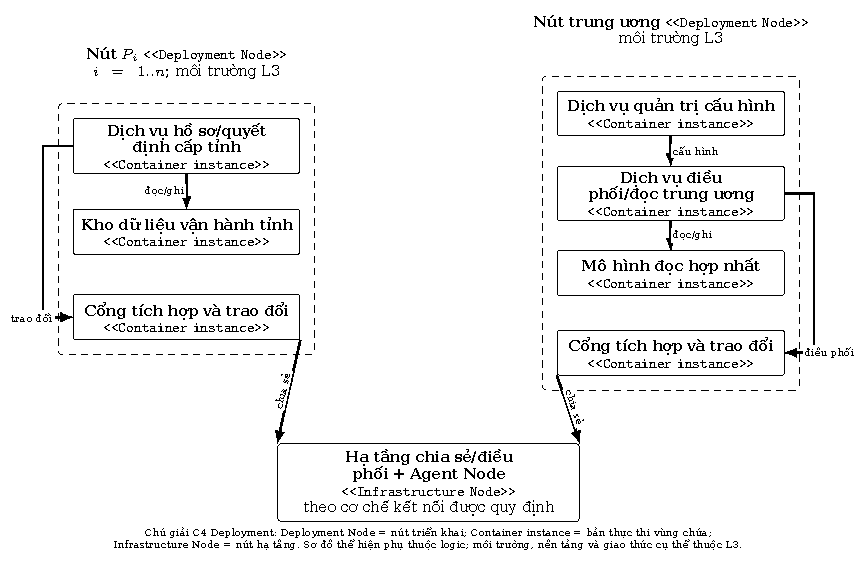
\includegraphics[width=0.94\textwidth]{figure_sources/fig05_c4_deployment_pdist.pdf}
\caption{Cấu hình triển khai logic P-DIST dùng cho stress-test; hạ tầng chia sẻ/điều phối và Agent Node là vai trò kết nối, không phải topology bắt buộc của SRA}
\label{fig:pdist-main}
\end{figure}

Trong ánh xạ này, ``Cổng tích hợp và trao đổi'' là vai trò logic của bộ thích nghi tích hợp. Khi hiện thực hóa trong hệ sinh thái Bộ Khoa học và Công nghệ, vai trò đó phải tương thích với lớp tích hợp, chia sẻ và điều phối của QĐ 1973 (LGSP/LDOP, API Gateway, Agent Node) và cơ chế kết nối qua Nền tảng chia sẻ, điều phối dữ liệu/Agent Node theo NĐ 278 \citep[Mục~III.1.4]{qd1973_2026} \citep[khoản~2 Điều~4; khoản~3 Điều~7]{nd278_2025}. Vì vậy, Hình~\ref{fig:pdist-main} là profile L2 phục vụ đánh giá kiến trúc, không phải sơ đồ triển khai chính thức hoặc cấu hình được các văn bản dẫn chiếu bắt buộc.

Tương tự, góc nhìn an toàn/riêng tư chỉ khóa các bất biến kiến trúc: xác thực theo nguồn phù hợp, ủy quyền theo vai trò và phạm vi, tách đặc quyền tỉnh--trung ương, kiểm soát trường dữ liệu được trao đổi, lưu nguồn gốc/phiên bản và bằng chứng gửi--nhận, cùng trách nhiệm kiểm toán. Các yêu cầu này được dẫn xuất từ NĐ 69, NĐ 278, Luật Bảo vệ dữ liệu cá nhân và NĐ 356 \citep{nd69_2024,nd278_2025,luatbvdlcn2025,nd356_2025}. Chúng không chứng minh rằng một hệ thống chưa triển khai đã đạt cấp độ an toàn thông tin, thông lượng, tính sẵn sàng hay thời gian phục hồi cụ thể; các thuộc tính đó phải được kiểm chứng trên hiện thực hóa thực tế. Ma trận biên tin cậy--kiểm soát chi tiết được cung cấp trong tài liệu bổ trợ.

Cuối cùng, biến thể địa phương được giới hạn ở bước nội bộ, vai trò phối hợp và biểu mẫu phụ trợ; không được thay đổi thẩm quyền, trạng thái quyết định hoặc thời hạn L1, và phải có phiên bản/ngày hiệu lực. Cấu trúc mô hình chung--biến thể địa phương phù hợp với tiền lệ về quy trình cấu hình trong chính quyền đô thị \citep[pp.~486--500]{gottschalk2009municipality}. Đồng thời, địa bàn được dùng để xác định thẩm quyền chứ không làm ranh giới của toàn bộ hệ sinh thái: quan hệ doanh nghiệp--quỹ--chuyên gia--viện/trường cần được lưu xuyên địa bàn \citep[pp.~27--28]{fischer2022}; \citep[pp.~1483--1484]{noak2025}.
